\definecolor{rktext}{RGB}{34,38,45}
\definecolor{rkmuted}{RGB}{101,109,120}
\definecolor{rkline}{RGB}{125,133,144}
\definecolor{rkred}{RGB}{214,67,78}
\definecolor{rkredfill}{RGB}{255,240,242}
\definecolor{rkblue}{RGB}{76,119,189}
\definecolor{rkbluefill}{RGB}{238,244,255}
\definecolor{rkgreen}{RGB}{68,148,116}
\definecolor{rkgreenfill}{RGB}{237,248,242}
\definecolor{rkorange}{RGB}{220,145,48}
\definecolor{rkorangefill}{RGB}{255,245,231}
\definecolor{rkgrayfill}{RGB}{243,246,249}

\begin{tikzpicture}[
  x=1cm,
  y=1cm,
  every node/.style={inner sep=0pt, outer sep=0pt},
  rkTitle/.style={font=\sffamily\bfseries\fontsize{11}{11.6}\selectfont, text=rktext},
  rkBoxTitle/.style={font=\sffamily\bfseries\fontsize{8.4}{9.0}\selectfont, text=rktext, align=center},
  rkText/.style={font=\sffamily\fontsize{6.5}{7.1}\selectfont, text=rkmuted, align=center},
  rkCenter/.style={rounded corners=0.16cm, line width=1.0pt, draw=rkred, fill=rkredfill},
  rkBlue/.style={rounded corners=0.14cm, line width=0.9pt, draw=rkblue, fill=rkbluefill},
  rkGreen/.style={rounded corners=0.14cm, line width=0.9pt, draw=rkgreen, fill=rkgreenfill},
  rkOrange/.style={rounded corners=0.14cm, line width=0.9pt, draw=rkorange, fill=rkorangefill},
  rkGray/.style={rounded corners=0.14cm, line width=0.9pt, draw=rkline, fill=rkgrayfill},
  rkArrow/.style={draw=rkline, line width=0.85pt, ->}
]

  \path[use as bounding box] (-0.08, 0.60) rectangle (11.84, 6.08);

  \begin{scope}[xshift=-0.65cm]
  \node[rkTitle] at (5.96, 5.86) {Key properties of a rootkit};

  % Top
  \draw[rkBlue] (3.28, 4.42) rectangle (8.48, 5.34);
  \node[rkBoxTitle, text=rkblue] at (5.88, 4.98) {Privilege and persistence};
  \node[rkText] at (5.88, 4.66) {maintains long-term control after intrusion};

  % Center
  \draw[rkCenter] (3.94, 2.58) rectangle (7.82, 4.14);
  \node[text=rkred] at (5.4, 3.6) {\fontsize{15}{15}\selectfont \faUserSecret};
  \node[rkBoxTitle, text=rkred] at (6.2, 3.5) {Rootkit};
  \node[rkText, text=rkred] at (5.96, 2.9) {malware that keeps privileged access\\and hides its presence};

  % Left and right
  \draw[rkGreen] (0.08, 2.92) rectangle (3.54, 3.98);
  \node[rkBoxTitle, text=rkgreen] at (1.81, 3.60) {Concealment};
  \node[rkText] at (1.81, 3.18) {hides files, processes\\connections or logs};

  \draw[rkOrange] (8.22, 2.92) rectangle (11.68, 3.98);
  \node[rkBoxTitle, text=rkorange] at (9.95, 3.60) {Hooking and tampering};
  \node[rkText] at (9.95, 3.18) {intercepts normal execution\\and alters returned data};

  % Bottom
  \draw[rkGray] (2.44, 0.72) rectangle (9.32, 1.78);
  \node[rkBoxTitle] at (5.88, 1.34) {Compromised system = untrusted view};
  \node[rkText] at (5.88, 0.98) {security tools above the attacker may receive manipulated information};

  % Arrows
  \draw[rkArrow] (5.88, 4.42) -- (5.88, 4.18);
  \draw[rkArrow] (3.54, 3.45) -- (3.88, 3.45);
  \draw[rkArrow] (8.22, 3.44) -- (7.88, 3.44);
  \draw[rkArrow] (5.88, 2.52) -- (5.88, 1.84);
  \end{scope}

\end{tikzpicture}
